\chapter{144.390MHz Channel Capacity}

One of the largest limitations of the APRS network is the fact that it primarily operates
on a single national data channel. Individual nodes share the 1200bps channel using 
CSMA as discused in section~\ref{sec:bell202csma}, but the relationship between 
these channel access methods and how often a station should beacon isn't straight-forward.

The APRS specification fails to give concrete guidance on what beacon interval should
be used beyond stating that every station should beacon at the net's cycle rate,
which it lists as 10 minutes direct and 30 minutes \cite[p.~9]{aprsspec}. 
For fixed nodes such as weather stations and network infrastructure, 
these intervals are appropriate, but mobile users find this beacon interval unsatisfying
and not useful. There is an almost universal desire to beacon more often than every 10 minutes,
but how often is allowable in the limitations of the network?

An appropriate starting point for analyzing APRS channel capacity would be the original methods
developed for the ALOHA System at the University of Hawaii
which APRS was originally based upon \cite{packetthroughput}.
The ALOHAnet was a 9600bps UHF packet radio system that was the first application of 
wireless computer networking. 
This system developed several of the shared channel access methods 
that would subsequenty be used in other protocols such as Ethernet, GSM, and APRS.

\section{Poisson Channel}

The most basic analysis of a channel's ALOHA capacity is based on the assumption that
each packet is the same length, that traffic enters the network as a Poisson process,
and that any collision between two packets causes both of them to fail to be delivered.
Defining the rate of packets entering the network as $\lambda$ in packets per second and
the length of each packet as $\tau$ in seconds, the normalized channel traffic G can be
calculated as
\begin{equation}
	G = \lambda \tau
\end{equation}
This normalized value idicates what fraction of a channel would be needed for all
of the traffic entering the network, so for example a value $G=1.0$ would indicate that
a single station would need to transmit packets continuously, where $G=0.5$ indicates 
a free channel half the time. 

Unfortunately, since channel access is stochastic, 
there is no guarantee that two stations won't transmit at the same time.
Any packet transmission starting less than $\tau$ seconds before or after another would
cause a collision and two lost packets. 
This indicates that the rate of successfully received packets exiting the network must
be lower than $\lambda$, and is traditionally notated as $\lambda'$. 
Since $\lambda' \leq \lambda$, we define the normalized channel throughput S as
\begin{equation}
	S = \lambda' \tau
\end{equation}
Due to the assumption that the channel access is Poisson, 
the probability that a packet will collide with another is $e^{-2 \lambda \tau}$,
which therefore yields the relationship between S and G of
\begin{equation}
	S = G e ^ {-2 G}
\end{equation}
This indicates a moderately surprising result that for Poisson channel access,
the throughput is completely independent of the number of stations on the channel,
but only dependent upon the total channel loading.

\begin{figure}
	\centering
	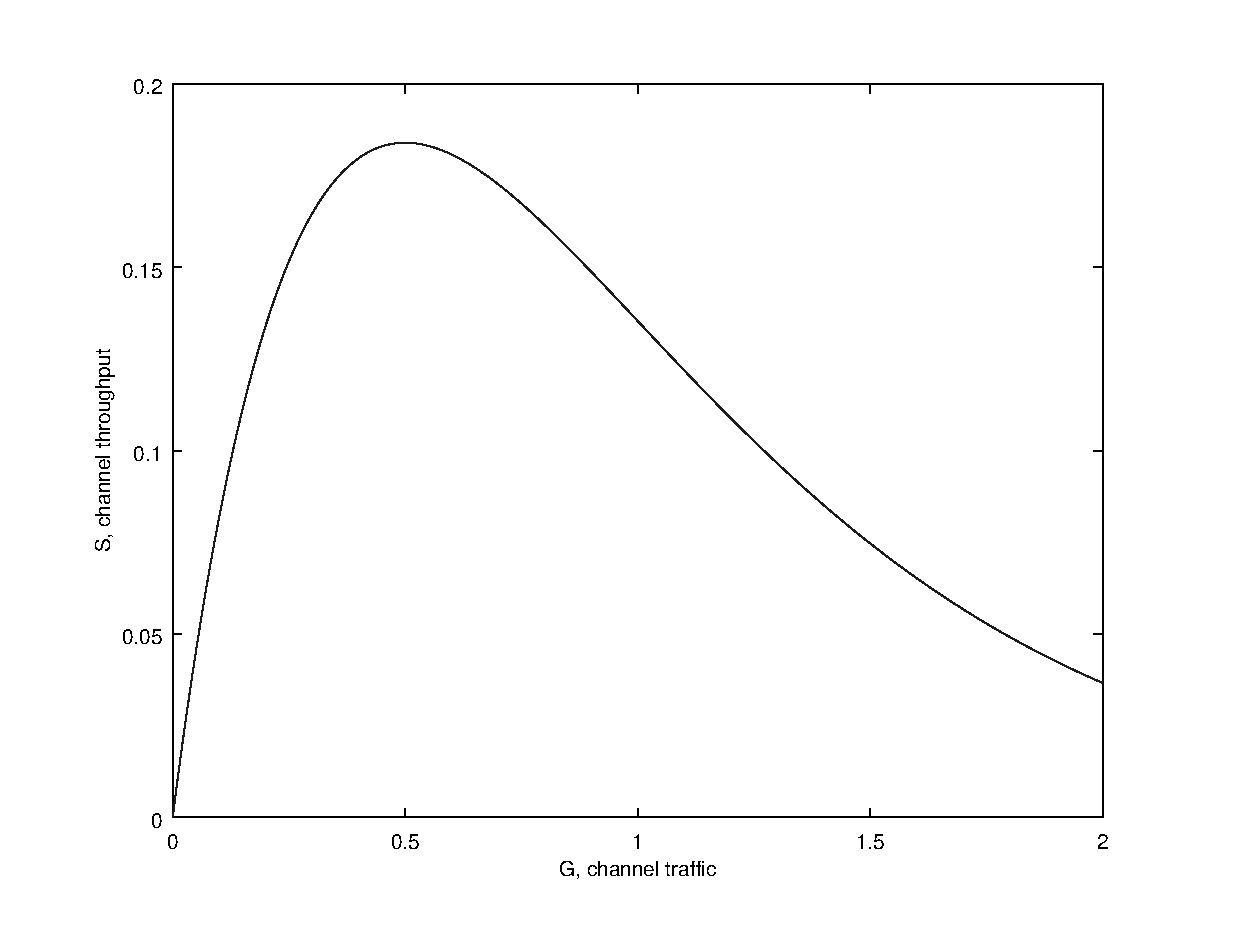
\includegraphics[width=1.0\textwidth]{src/octave/poissonthroughput}
	\caption{Poisson channel traffic and throughput}
	\label{fig:SGpoisson}
\end{figure}
Graphing the channel throughput versus the channel's traffic yields figure 
\ref{fig:SGpoisson}, which indicates that as you increase channel traffic, 
throughput increases to a point when packet collisions finally start to dominate
the channel and throughput starts to roll off again. This inflection point is at
a channel traffic $G = 0.5$ at which point 36\% of the packets are expected
to be successfully decoded.

While assuming that APRS traffic is based on a Poisson process is 
highly suspect, this simple model of channel capacity does yield some insightful 
values. 
Collecting several days of APRS traffic on 144.390MHz in San Luis Obispo
shows an average packet size of 119 octets. With a typical 300ms preamble
and a data rate of 1200bps, this yields $\tau = 1.09$.
\begin{equation}
	\lambda_{APRS} = \frac{G_{MAX}}{\tau} = 0.457
	\label{equ:aprsmaxrate}
\end{equation}

Equation \ref{equ:aprsmaxrate} indicates that a single APRS channel can support
27 transmitted packets per minute, which need to be apportioned to 
all of the participating network nodes. 
Assuming the typical target LAN size of 60 stations, 
this implies an average beacon interval per station of \emph{2 minutes 13 seconds}.
The less satisfying result is the fact that only 10 of these packets will be 
successful received, which indicates that
two thirds of the transmitted power is wasted.

\section{Deficiencies of the Poisson Model}

There were several assumptions made to simplify the just-presented model 
for an ALOHA channel that are not particularly valid 
when applied to a typical APRS network. 
While most of these assumptions indicate that the result of
equation \ref{equ:aprsmaxrate} is overly optimistic, there is enough conflict 
that the true traffic versus throughput relationship isn't easily found.

Most glaringly, this initial model ignores any kind of collision avoidance 
between stations. While deaf APRS trackers are not unusual, a large fraction
of trackers do support CSMA, which would ensure that a collision would
only happen if both stations started transmitting within the preamble time of
each other, not the entire packet length. Should a station decide to
transmit when it can hear that the channel is already busy, it is expected to
hold off transmitting until the channel goes clear. This reduces the window
of possible collisions from the entire length of the packet to only the 
length of the preamble and would increase channel throughput.

Opposingly, this model ignores the effect of digipeaters on each packet's
effective length on the channel. Each packet is multiplied by the number of
hops requested, causing a single packet to occupy several consecutive time slots.
This would indicate that stations would need to beacon on a much longer interval
to keep their average packet rate below the channel's optimal level.
Unfortunately, the digipeaters are also one of the most concrete examples of how
invalid the Poisson distribution assumption is for the channel. 
Poisson distributions require that the process is memoryless, but digipeaters
imply that a large fraction of traffic on the channel isn't caused by independent events
but by immediately prior events on the same channel. This causes APRS traffic to
be what's called a self-similar process. This property has been widely studied 
since TCP/IP Poisson traffic models suffer from the same deficiency \cite{failureofpoisson}. 
Applying the traffic models developed for the Internet Protocol to APRS 
would likely yield several insightful results, but is beyond the scope of this work.


